


\setcounter{page}{1}

\chapter{Introduction}
Since the 1980's, {\gls{uav}}'s have been a subject of interest for the military. Up until the early/mid 1990's the technology required to implement these Unmanned Vehicles was not available. Today with the advance of miniaturization, more powerful processors and more reliable sensors it is finally possible to produce such devices. As sensors and micro-processors  became more viable the interest in \gls{vtol} aircrafts increased. Hence, universities began to invest in the research of quad-rotors/helicopters due to their advantage over traditional fixed-wing crafts. \gls{vtol} are more advantageous in the following situations: rescue operations, delivery of goods, maneuvering in enclosed spaces. The military's interest in these devices stems from their high maneuverability even in minute form while still maintaining the ability to carry significant payloads, which makes them prime candidates for aerial surveillance and monitoring.

\section{History}
Despite the recent development and interest in the quad-rotor the concept is not new; the first idea for a quad-rotor was developed in 1907 by Louis and Jacques Breguet and was called the “Gyroplane No.1” (see figure \ref{fig:Gyroplane No.1}) \cite{Principles_of_helicopter_aerodynamics}.  The quad-rotor was propelled by four rotors with 4-blades mounted on the extremities of a cross-shaped structure. To cancel the rotational torques the rotorcraft used diagonally opposed rotors which rotate in opposite direction, the same theory is used in the quad-rotor featured in this report. Even though the rotorcraft achieved lift for a sustained period it could not remain stable enough to consider it a flight. It would take another 50 years for both the control theory and technology to catch up to this revolutionary idea, and allow the first actual flight of a quad-rotor.

\begin{figure}[h]
	\centering
	\begin{subfigure}[b]{0.35\textwidth}
		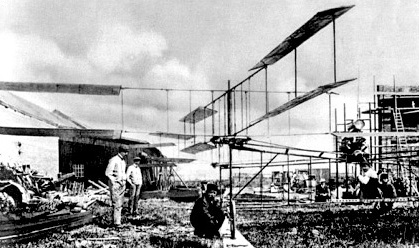
\includegraphics[width=\textwidth]{\DocRoot/images/breguet_gyro_1}
		\caption{Gyroplane No.1}
		\label{fig:Gyroplane No.1}
	\end{subfigure}%
	~ %add desired spacing between images, e. g. ~, \quad, \qquad, \hfill etc.
	%(or a blank line to force the subfigure onto a new line)
	\begin{subfigure}[b]{0.3\textwidth}
		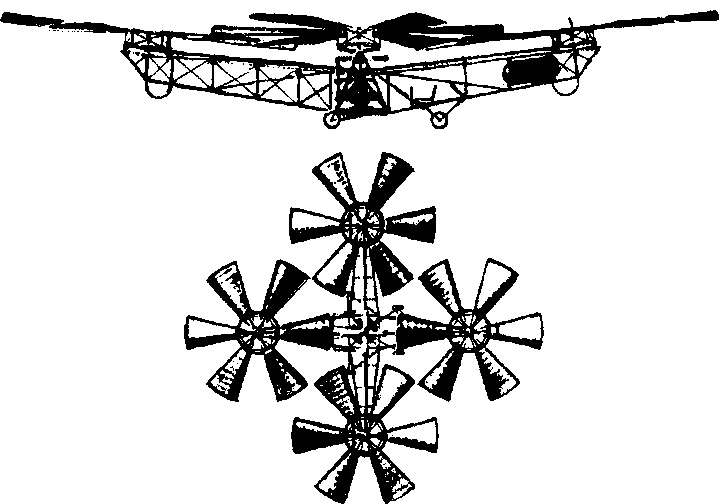
\includegraphics[width=\textwidth]{\DocRoot/images/bothezat_quad}
		\caption{Bothezat’s sketch}
		\label{fig:Bothezat’s sketch}
	\end{subfigure}
	~ %add desired spacing between images, e. g. ~, \quad, \qquad, \hfill etc.
	%(or a blank line to force the subfigure onto a new line)
	\begin{subfigure}[b]{0.3\textwidth}
		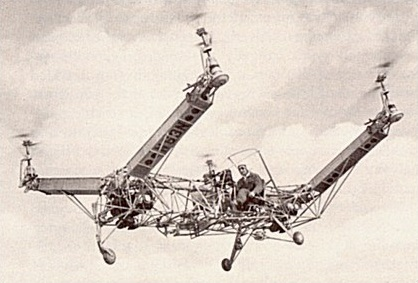
\includegraphics[width=\textwidth]{\DocRoot/images/convertawings}
		\caption{Convertawings Model A}
		\label{fig:Convertawings Model A}
	\end{subfigure}
	\caption{Development of the Quad-rotor concept \cite{Principles_of_helicopter_aerodynamics}}\label{fig:Development of the Quad-rotor concept}
\end{figure}


In  1921, the US Air Corps awarded a contract to Dr. George de Bothezat and Ivan Jerome to work on a vertical flight machine (see figure \ref{fig:Bothezat’s sketch}) \cite{Principles_of_helicopter_aerodynamics}. The result was a four six-bladed quad-rotor mounted at the ends of beams 20 metres in length arranged in a cross like structure. The craft overcame the stability problems present in quad-rotor built up until then by using two variable pitch controlled to ensure stability and control the craft. It was the first craft to prove that vertical flight  was possible despite it's limited reach of only 5 meters.

Due to stability problems the quad-rotor design   was abandoned in favour of research of the now traditional helicopter. It wasn't until 1956 that the concept of the quad-rotor was once again modernized with the “Convertawings Model A” \cite{Helicopters_and_autogiros(Convertawings_Model_A)} (see figure \ref{fig:Convertawings Model A}) whose development greatly improved the four rotor aircraft built by Oehmichen and Bothezat. With a simplified control system and greater power than its predecessors it was the first quad-rotor to fly successfully.


As a result of military interest the quad-rotor has been studied extensively as an alternative to traditional helicopters which were capable of carrying large payloads. The current and most widely known quad-rotor is the 2006 “Bell Boeing Quad Tilt-Rotor” (seen in figure \ref{fig:Bell Boeing Quad TiltRotor}), which was based on the two “Curtiss-Wright X-19” and “Bell X-22”  (see figures \ref{fig:Curtiss-Wright X-19.} and \ref{fig:Bell X-22.} respectively) which were two prototype quad-rotors built in the 1960's. The Bell Boeing Quad Tilt-Rotor was designed for military use to transport cargo of up to 9000kg to otherwise unreachable locations.   


\begin{figure}[h]
	\centering
	\begin{subfigure}[b]{0.35\textwidth}
		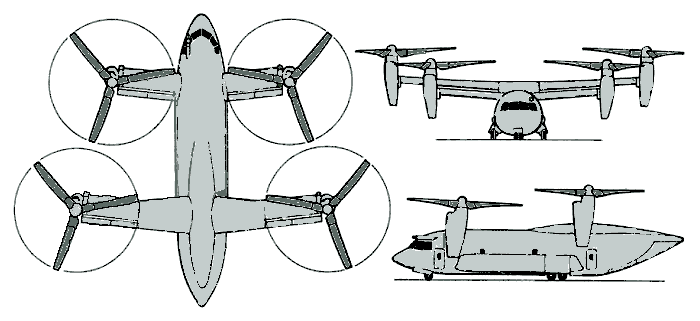
\includegraphics[width=4cm, height=3cm]{\DocRoot/images/QTRMV-44colour-1}
		\caption{Bell Boeing Quad Tilt-Rotor.}
		\label{fig:Bell Boeing Quad TiltRotor}
	\end{subfigure}%
	~ %add desired spacing between images, e. g. ~, \quad, \qquad, \hfill etc.
	%(or a blank line to force the subfigure onto a new line)
	\begin{subfigure}[b]{0.3\textwidth}
		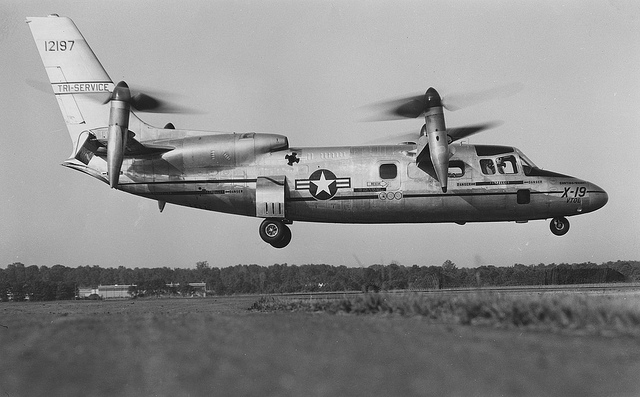
\includegraphics[width=4cm, height=3cm]{\DocRoot/images/6847501354_22de7e3548_z}
		\caption{Curtiss-Wright X-19.}
		\label{fig:Curtiss-Wright X-19.}
	\end{subfigure}
	~ %add desired spacing between images, e. g. ~, \quad, \qquad, \hfill etc.
	%(or a blank line to force the subfigure onto a new line)
	\begin{subfigure}[b]{0.3\textwidth}
		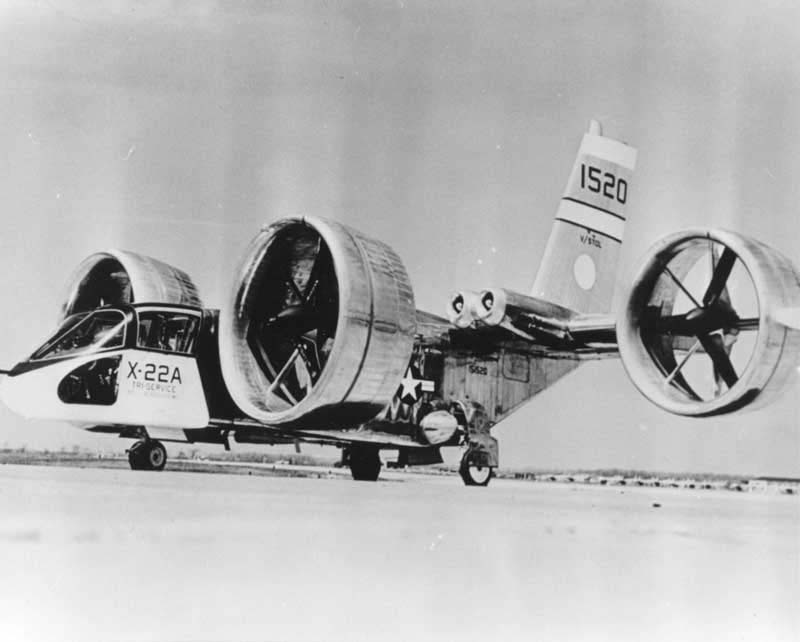
\includegraphics[width=4cm, height=3cm]{\DocRoot/images/X-22a_onground_bw}
		\caption{Bell X-22.}
		\label{fig:Bell X-22.}
	\end{subfigure}
	\caption{Further Development of the Quad-rotor Concept \cite{Principles_of_helicopter_aerodynamics}}\label{fig:Further Development of the Quadrotor Concept}
\end{figure}


Today, major breakthroughs in the concept of the quad-rotor have taken place in universities across the world. Examples of such break through are as follows; comparison of fixed-pitch and variable-pitch propeller based quad-rotors,  the development of  a robust controllers and test of a trajectory algorithm for variable-pitch aircrafts as seen in \cite{Variable_Pitch_Quadrotor_MIT, comparison_of_fixed_and_variable_pitch_actuators}. A paper written by a Czech researcher was found which develops an \gls{ekf} along with a \gls{lqr} based control system for a quad-rotor which was used to adequately control the system\cite{identification_and_Control_of_a_Quadrotor_(czech)}. In MIT a prototypes have been  developed  that are capable of exciting flips, and peak rotational rates exceeding $1600^{\circ}s^{-1}$ were accomplished using traditional fixed-pitch technology \cite{high_speed_quadrocopter_multi_flips}. Research groups have developed prototypes that can fly through windows and narrow gaps and perch on inverted surfaces \cite{Quad_fly_through_windows}. A group in ETH zurich are now combining the quad-rotor with traditional control problems such as the inverted pendulum \cite{flying_inverted_pendulum}. Other research personnel are currently focusing on mapping of areas using \gls{slam} and streaming the results to a a remote computer \cite{mapping_quad}. Note the improvement of the quad-rotors are not just limited to the military and academia; some hobbyists have developed \gls{rc} variable-pitch quad-rotors and have posted their findings on \gls{rc} forums and discussion boards \cite{misc_video}.

\begin{comment}
\section{Project Goals}
A benefit of doing a project in this area is the vast amount of information available about the subject of autonomous flight and the control/simulation of quad-rotors. 
The primary goal was to obtain a deeper understanding of control techniques, how one would implement them on a chip and improve programming skills in the process. The group's objective, was to control the quad-rotor in the hovering position in a certain location by using the supplied digital sensors \cite{accelerometer_datasheet,compass_datasheet,gyroscope_datasheet,rangefinder_datasheet,GPS_datasheet} and implement obstacle avoidance if possible. The main target was to obtain a complete and realistic control system for the quad-rotor with complete documentation so that the quad-rotor can be utilized in future projects/studies. 
\end{comment}


\chapter{Ethics}
Over the recent years quad-rotors have found use in many areas some of which have raised ethical issues. Currently, there are numerous ethical problems, primarily flying quad-rotors in urban areas. For most parts these devices have to abide by the same restrictions as \gls{rc} planes, i.e  to be flown below a maximum of 120 m, 150 m from other people and the operator has to maintain line of sight at all times \cite{quad_fly_ireland}. For research and commercial use written permission from the national aviation regulator is often required. Today, many hobbyists fly quad-rotors over urban areas: hobbyists feel they should be allowed to fly where they like (even with a camera on board) while the public want to maintain their privacy. 
Many quad-rotors sold to hobbyists some with holsters for a camera which are used to shoot video while in flight. The general public are very concerned about how this impacts privacy \cite{Consumer_drones}. Clear and well though out rules must be designed to deal with this issue. 
Due to this privacy issue there have been numerous bills passed in order to deal with this growing problem\cite{Quadcopters_Cameras}.



Certain companies have taken an interest in quad-rotors due to their capabilities to navigate urban areas with ease. Amazon and Google use programs based around quad-rotors delivering items \cite{amazon_drones}. Certain medical services are interested in drones to facilitate organ implants to remote locations as they can reach higher speeds, thus,  allowing more lives to be saved \cite{quad_ieee_med}. The concept of \gls{uav} is also being used to help herd cattle in remote locations in Australia  \cite{herding_video}. As a result of large companies investing in quad-rotors to such a large degree some people (couriers) are worried that they could loss their jobs to a quad-rotor. 

The military's interest in drones has driven the development of the quad-rotor to the level it is a today. The reasons the military have invested in such a platform such ass this must be considered when undertaking a dual use technology like this project  Since the conception of the quad-rotor the military have shown great interest because of its potential to reach difficult locations and their lifting capability, which can be seen from the development of the  “Bell Boeing Quad Tilt-Rotor”.  But more recently these drones have been used by the US and Israeli army for surveillance and there have been rumours/videos of quad-rotors being used as tactical weaponry \cite{quad-rotor_with_Machine_Gun, Armed_Quadrotors}. 

This potential dual use  means this project could be used to help or hinder the progress of mankind.